\documentclass{article}
%\usepackage{tex4ht}
\usepackage{amsmath}
\usepackage{amsfonts}
\usepackage{amssymb}
\usepackage{amsthm}
\usepackage{graphicx}
\usepackage{color}
\usepackage{float}
\usepackage{dsfont}
\setlength{\parskip}{0.5\baselineskip}
\author{Zhuo Liu (0983311)}
\title{Project on Automatic Learning (Phase 2, Part 3)}
\date{March 4, 2014}

\definecolor{lightgray}{gray}{0.5}


\begin{document}
\maketitle


\section{Introduction}

In this report, similar to Part 2, we will apply kernel PCA to the large and small data
sets, to obtain KPC spaces, and then apply LDA on these KPC spaces to build classifiers. Since kernel PCA is nonlinear, the
classifier we build will be also nonlinear classifier. The difference from Part 2 is that the kernel we use in KPCA will become polynomial kernel, i.e.
\begin{equation}
 k(x,y) = (1+<x,y>)^{r}
\end{equation}
Still, the accuracy on both training and test set will be provided, and we can compare the result to the one in Part 2. (Here, we need to determine
the degree $r$ in (1). By several test, when $r=2$, we will get the best result. I think the reason is that large $r$ tends to overfit the problem.) 

%%% ------------------------------------------------------------------------------
\goodbreak

\section{Database: the Large One}

We will check the accuracy of the classifier build from LDA on the kernel PC space. The requirement of the kernel PC space is that 
90 percent of energy will be kept, i.e. we will keep k largest eigenvalues of covariance matrix, s.t.
\begin{equation}
 \frac{\sum_{i=1}^{k}\lambda_{i}}{\sum_{i=1}^{N}\lambda_{i}} > 0.9
\end{equation}
Figure 1 shows the spectrum for the kernel PCA matrix when the size of training set is $\frac{2}{3}$ of the whole set.

\begin{figure}[htp]
\centering
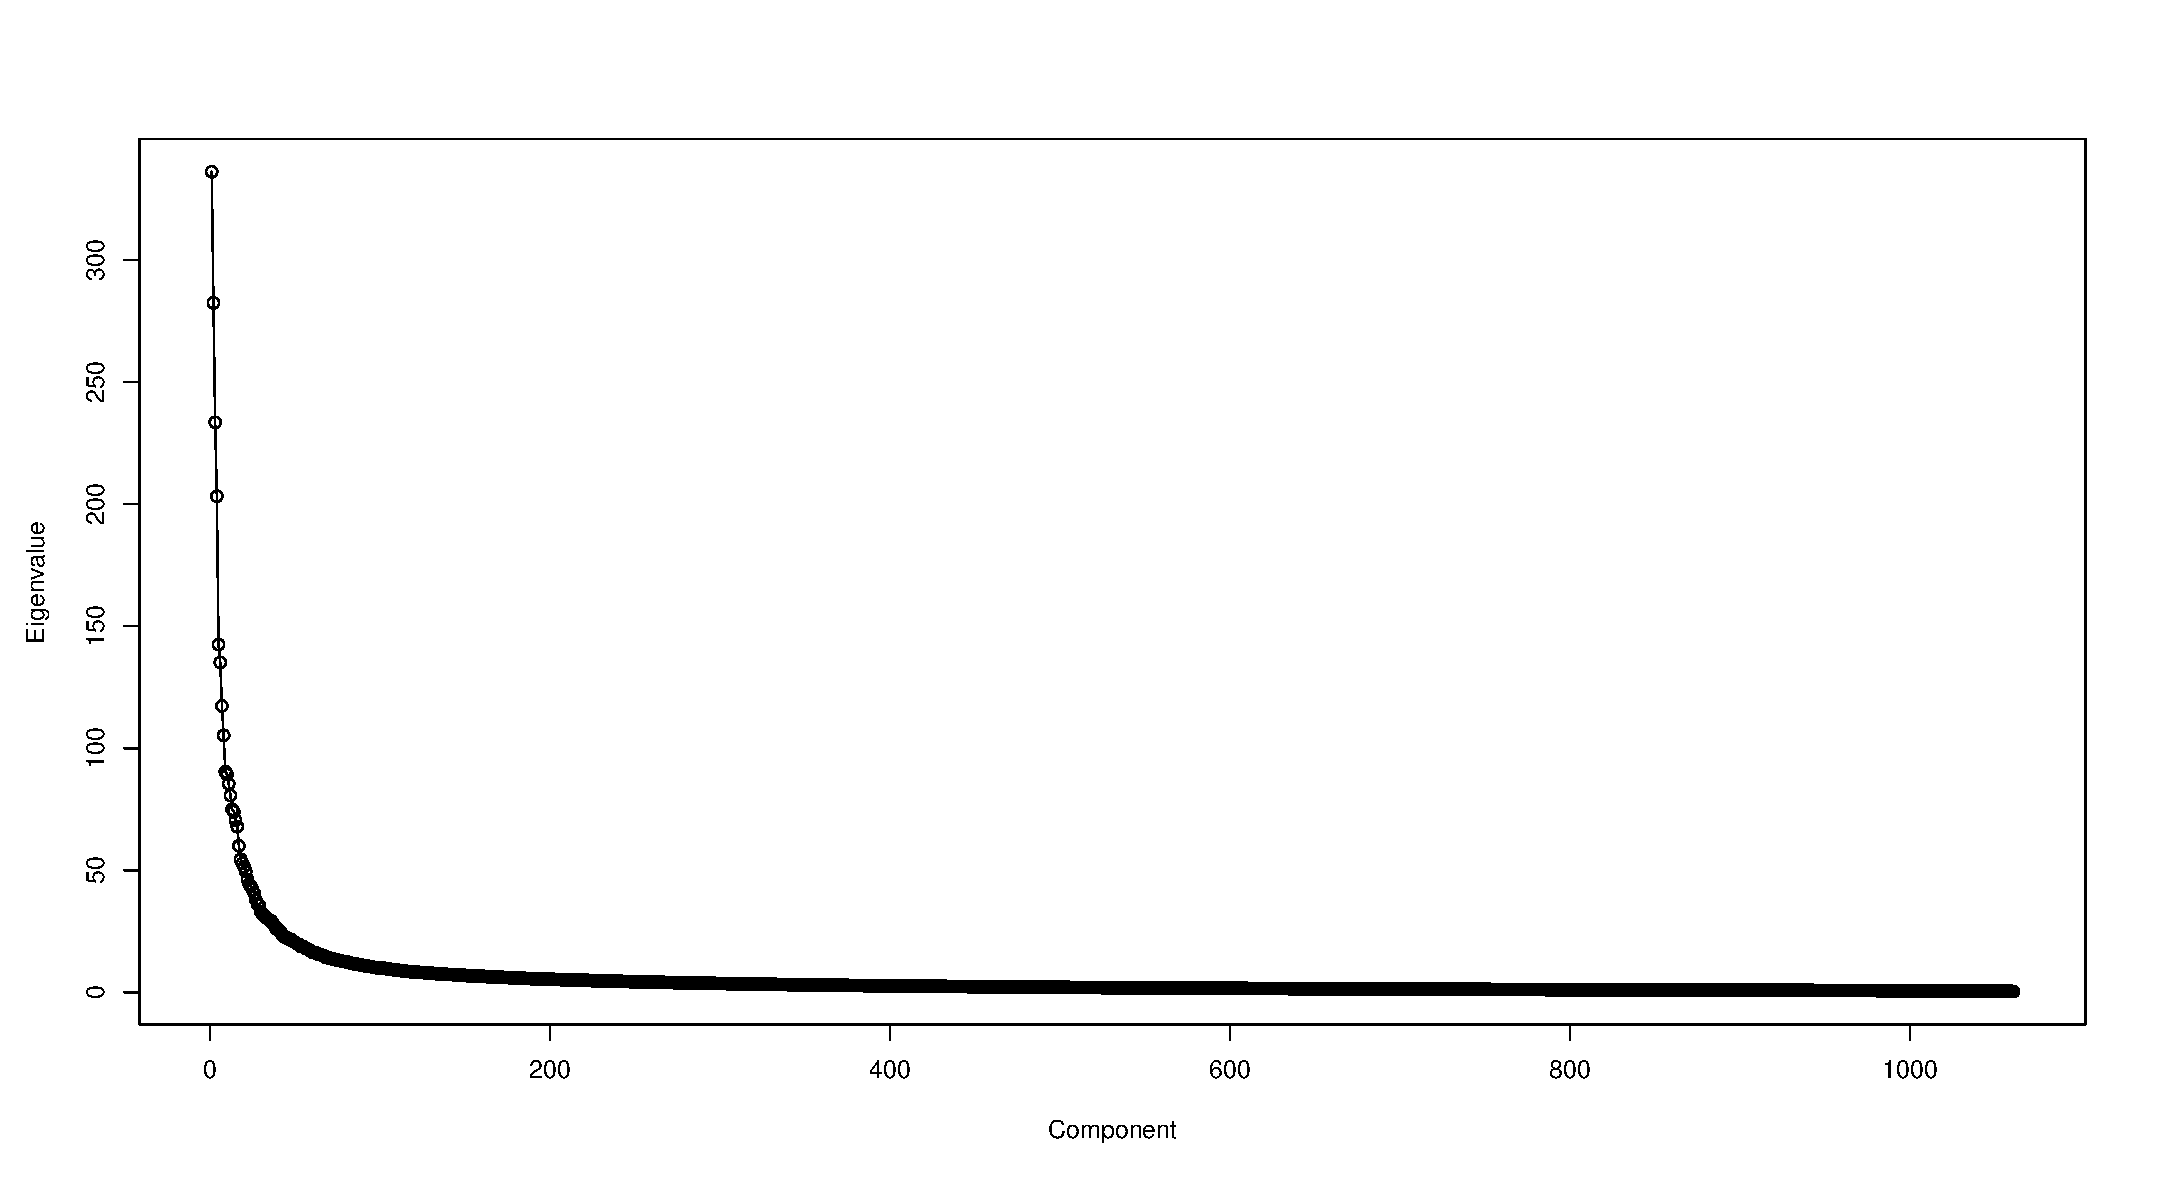
\includegraphics[width=12.1cm]{large_kpca_spectrum_poly.eps}
\caption{\textit{Spectrum for kernel PCA matrix (large data set)}}
\end{figure}

Similar to Part 2, we randomly choose training sets 9 times, whose sizes are $10\%$,$20\%$,...,$90\%$ 
of whole data set, and the remaining data compose the test set. The following table shows the accuracy of the non-linear classifier:

\scalebox{0.88}{
 \begin{tabular}{|c|c|c|c|}
  \hline
  Size of Traing Set  & Number of KPCs & Acc. on Training Set & Acc. on Test Set \\ \hline
  $10\%$              & 108            & 0.9937107            & 0.8131102        \\ \hline
  $20\%$              & 195            & 0.9937107            & 0.8831373        \\ \hline
  $30\%$              & 273            & 0.9958071            & 0.9041219        \\ \hline
  $40\%$              & 346            & 1.0000000            & 0.9435146        \\ \hline
  $50\%$              & 411            & 1.0000000            & 0.9585947        \\ \hline
  $60\%$              & 469            & 1.0000000            & 0.9529781        \\ \hline
  $70\%$              & 525            & 0.9991031            & 0.9456067        \\ \hline
  $80\%$              & 573            & 0.9992151            & 0.9529781        \\ \hline
  $90\%$              & 620            & 1.0000000            & 0.9500000        \\ \hline
 \end{tabular}
}
 
Figure 2,3 show the data projected on the first two and second two LD components space.

\begin{figure}[htp]
\centering
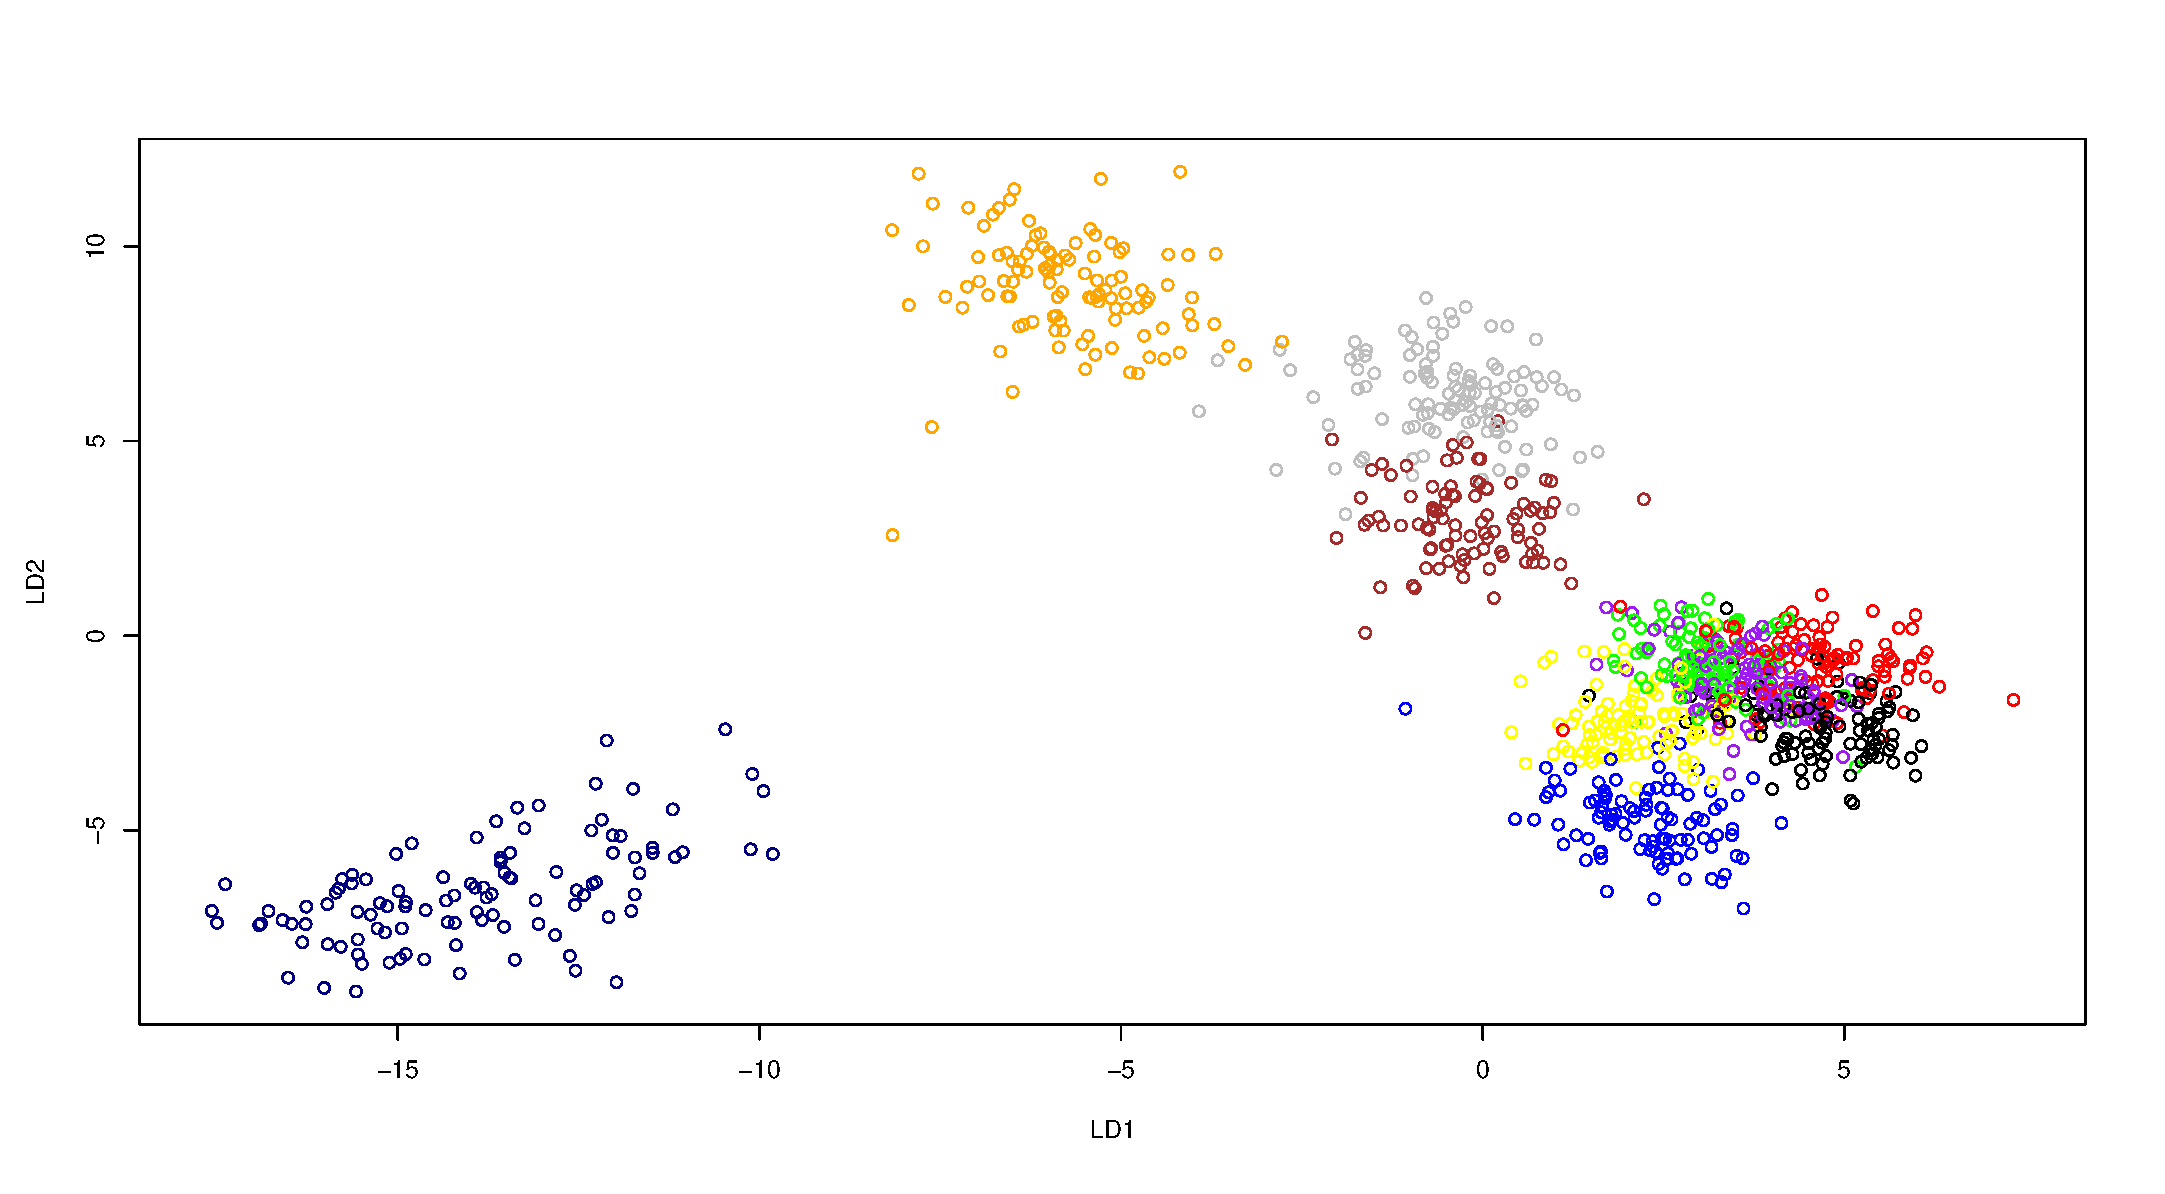
\includegraphics[width=12.1cm]{large_kpca_lda_poly_LD12.eps}
\caption{\textit{Projection of kernel PC space onto first two LD componets space (large data set). Here, the colors represent different classes: navy--0, green--1, 
blue--2, black--3, grey--4, brown--5, orange--6, purple--7, yellow--8, red--9.}}
\end{figure}

\begin{figure}[htp]
\centering
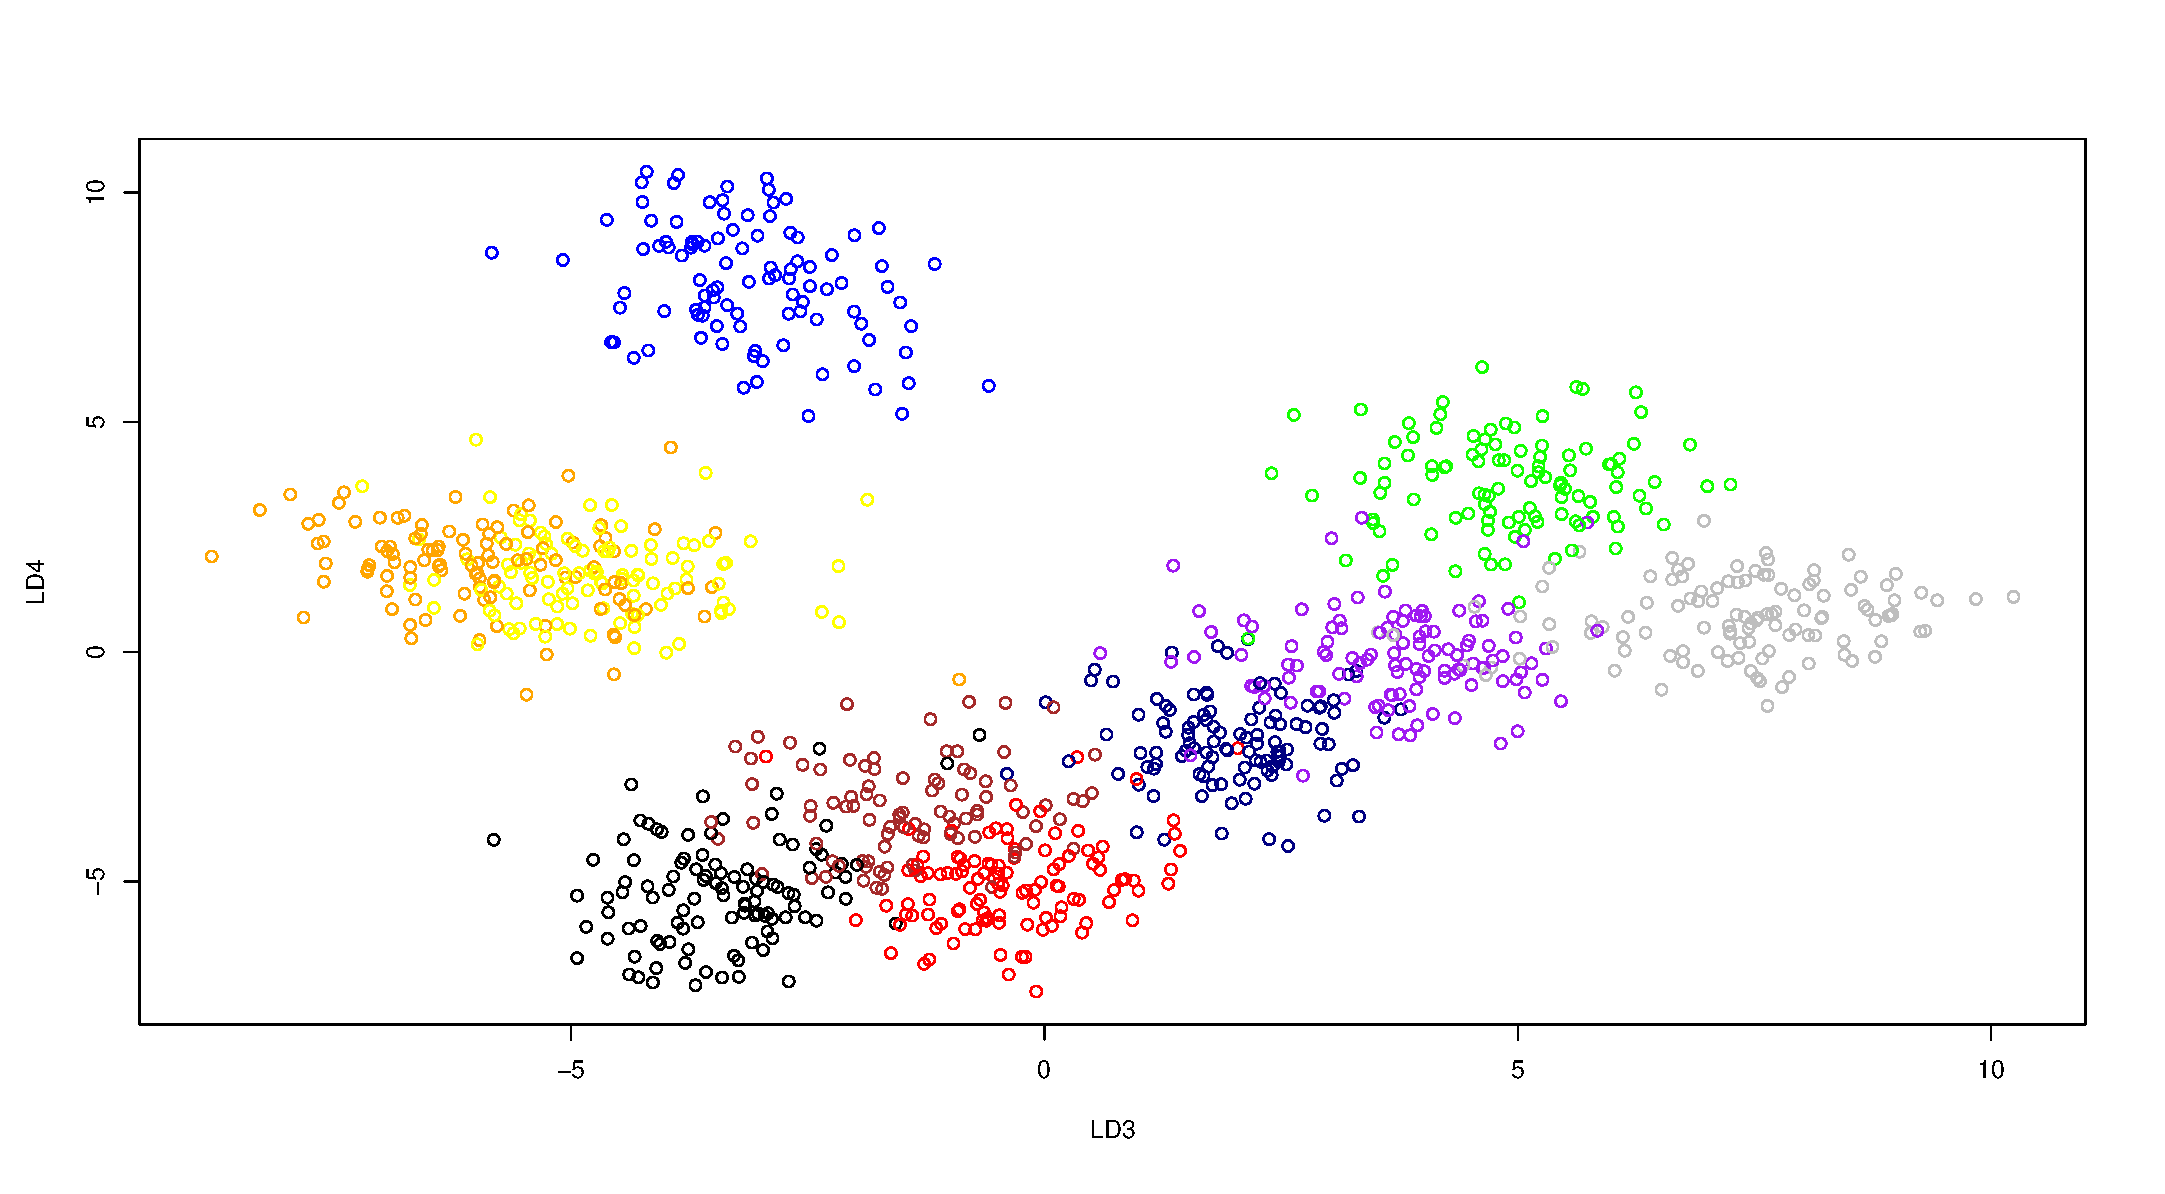
\includegraphics[width=12.1cm]{large_kpca_lda_poly_LD34.eps}
\caption{\textit{Projection of kernel PC space onto second two LD components space (large data set). Here, the colors represent different classes: navy--0, green--1, 
blue--2, black--3, grey--4, brown--5, orange--6, purple--7, yellow--8, red--9.}}
\end{figure}

By doing kernel trick, the obeservations in different classes are well separated, and we can easily build a linear classifier on this space.
Therefore, the above result is better than the one from linear classifier build on PC space in Part 2.

%%% ------------------------------------------------------------------------------
\goodbreak

\newpage

\section{Database: the Small One}

Similar to the procedure for large data set, first we will show in Figure 4 the spectrum for the kernel PCA matrix when the size of training set 
is $\frac{2}{3}$ of the whole set:

\begin{figure}[htp]
\centering
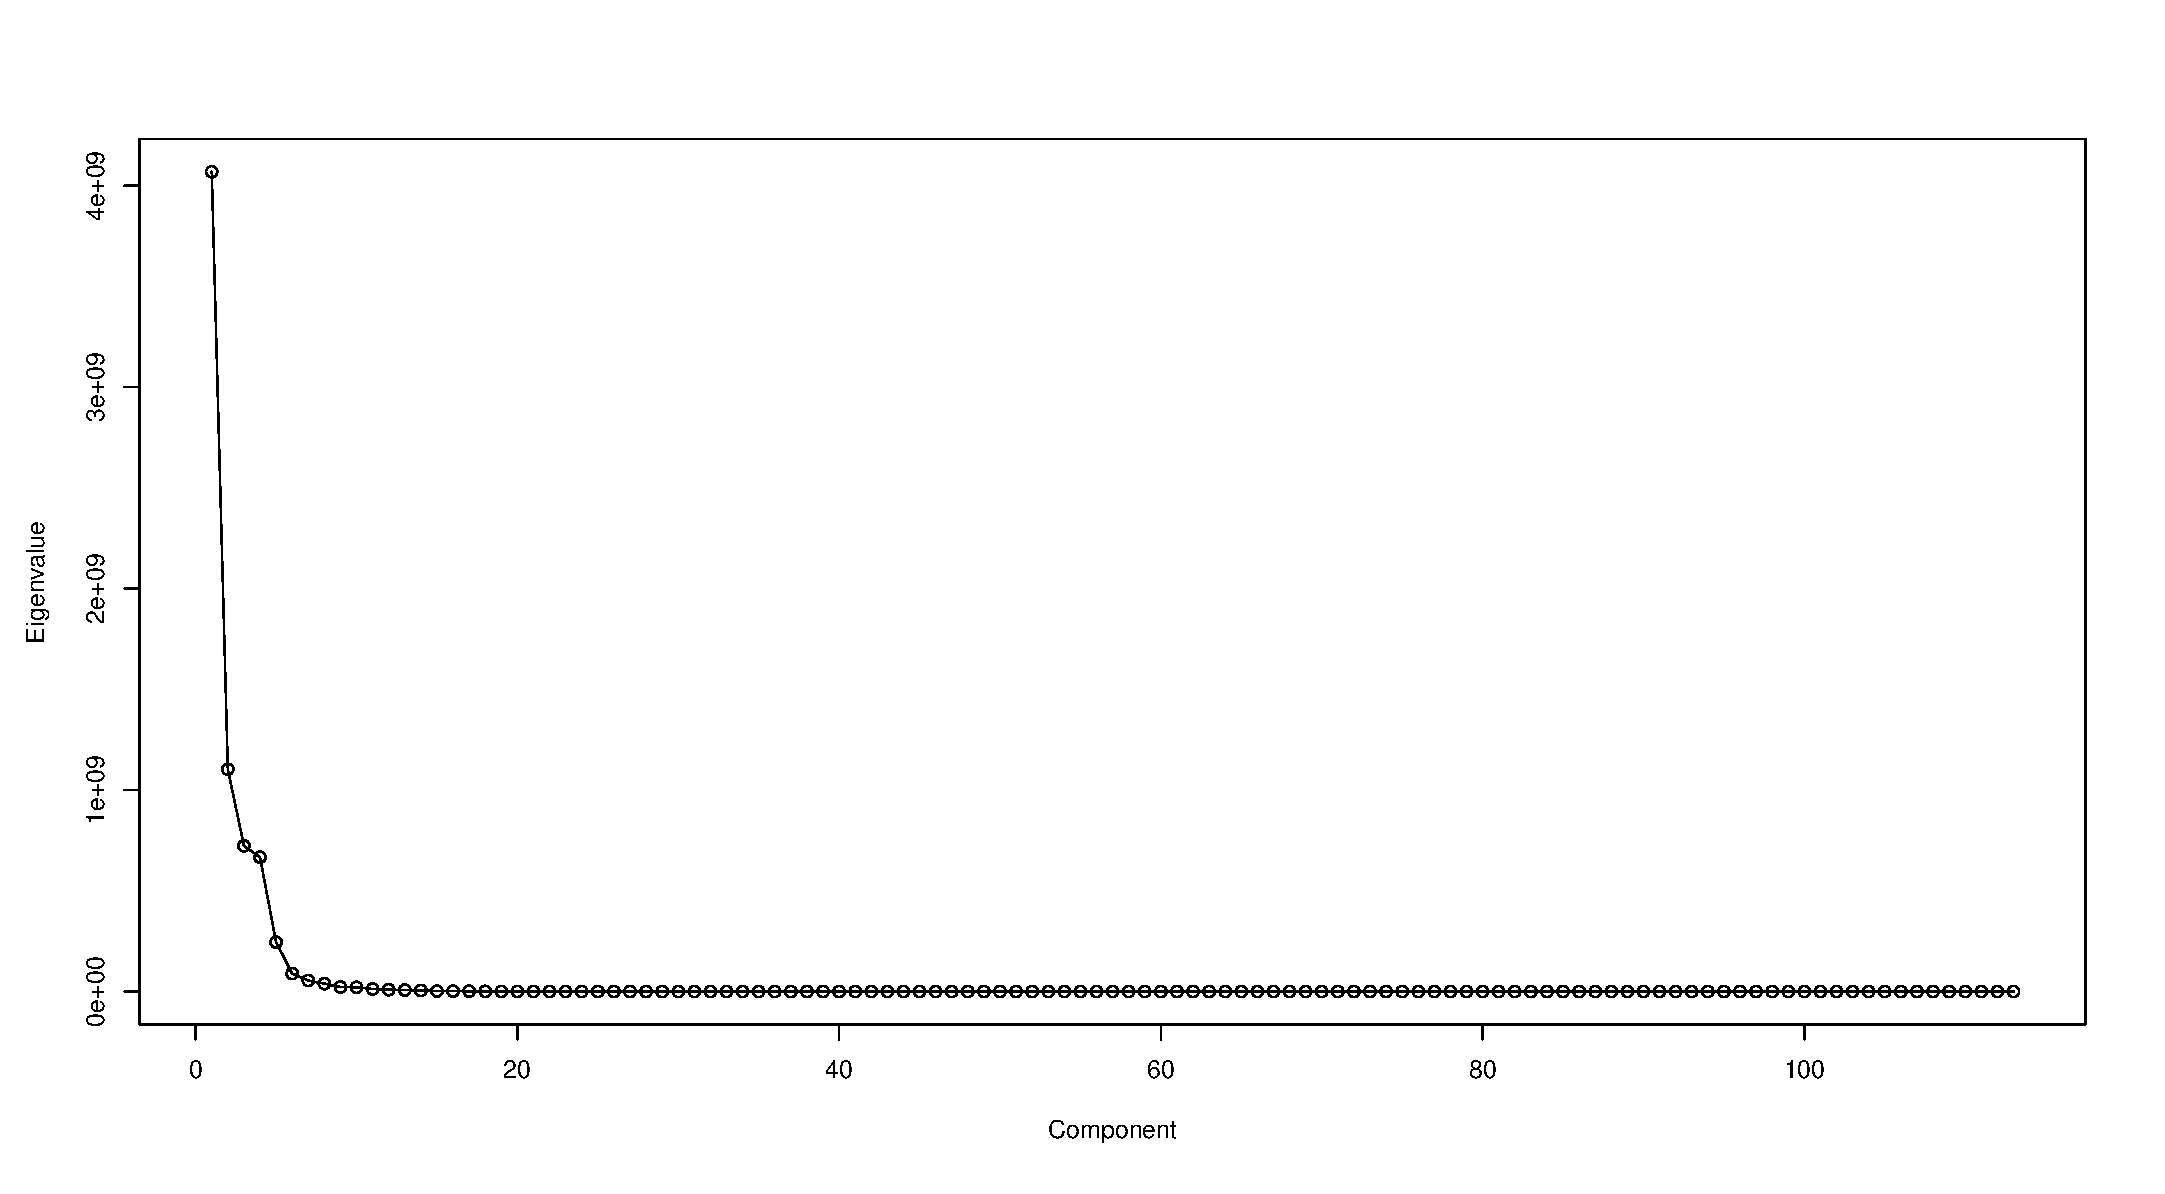
\includegraphics[width=12.1cm]{small_kpca_spectrum_poly.eps}
\caption{\textit{Spectrum for kernel PCA matrix (small data set)}}
\end{figure}

The following table shows the accuracy of the classifier build from kernel PC space which keeps $90\%$ of energy:

\scalebox{0.88}{
 \begin{tabular}{|c|c|c|c|}
  \hline
  Size of Traing Set  & Number of KPCs  & Acc. on Training Set & Acc. on Test Set \\ \hline
  $10\%$              & 3               & 0.7532468            & 0.7162097        \\ \hline
  $20\%$              & 2               & 0.4177489            & 0.4345238        \\ \hline
  $30\%$              & 3               & 0.5873016            & 0.5621521        \\ \hline
  $40\%$              & 4               & 0.5865801            & 0.5627706        \\ \hline
  $50\%$              & 4               & 0.5861472            & 0.5774892        \\ \hline
  $60\%$              & 4               & 0.5555556            & 0.5681818        \\ \hline
  $70\%$              & 4               & 0.5646259            & 0.5497835        \\ \hline
  $80\%$              & 4               & 0.5708874            & 0.5454545        \\ \hline
  $90\%$              & 4               & 0.5699856            & 0.5541126        \\ \hline
 \end{tabular}
}
 
Fiugre 5 shows the data projected on the first two LD components space. From this figure, we can find that polynomial kernel does not perform well
in this data set, because data is still not well seperated as in PC space. As a result, the accuracies on both training and test set are not so
good. Therefore, polynomial kernels have limitations for some problems.

\begin{figure}[htp]
\centering
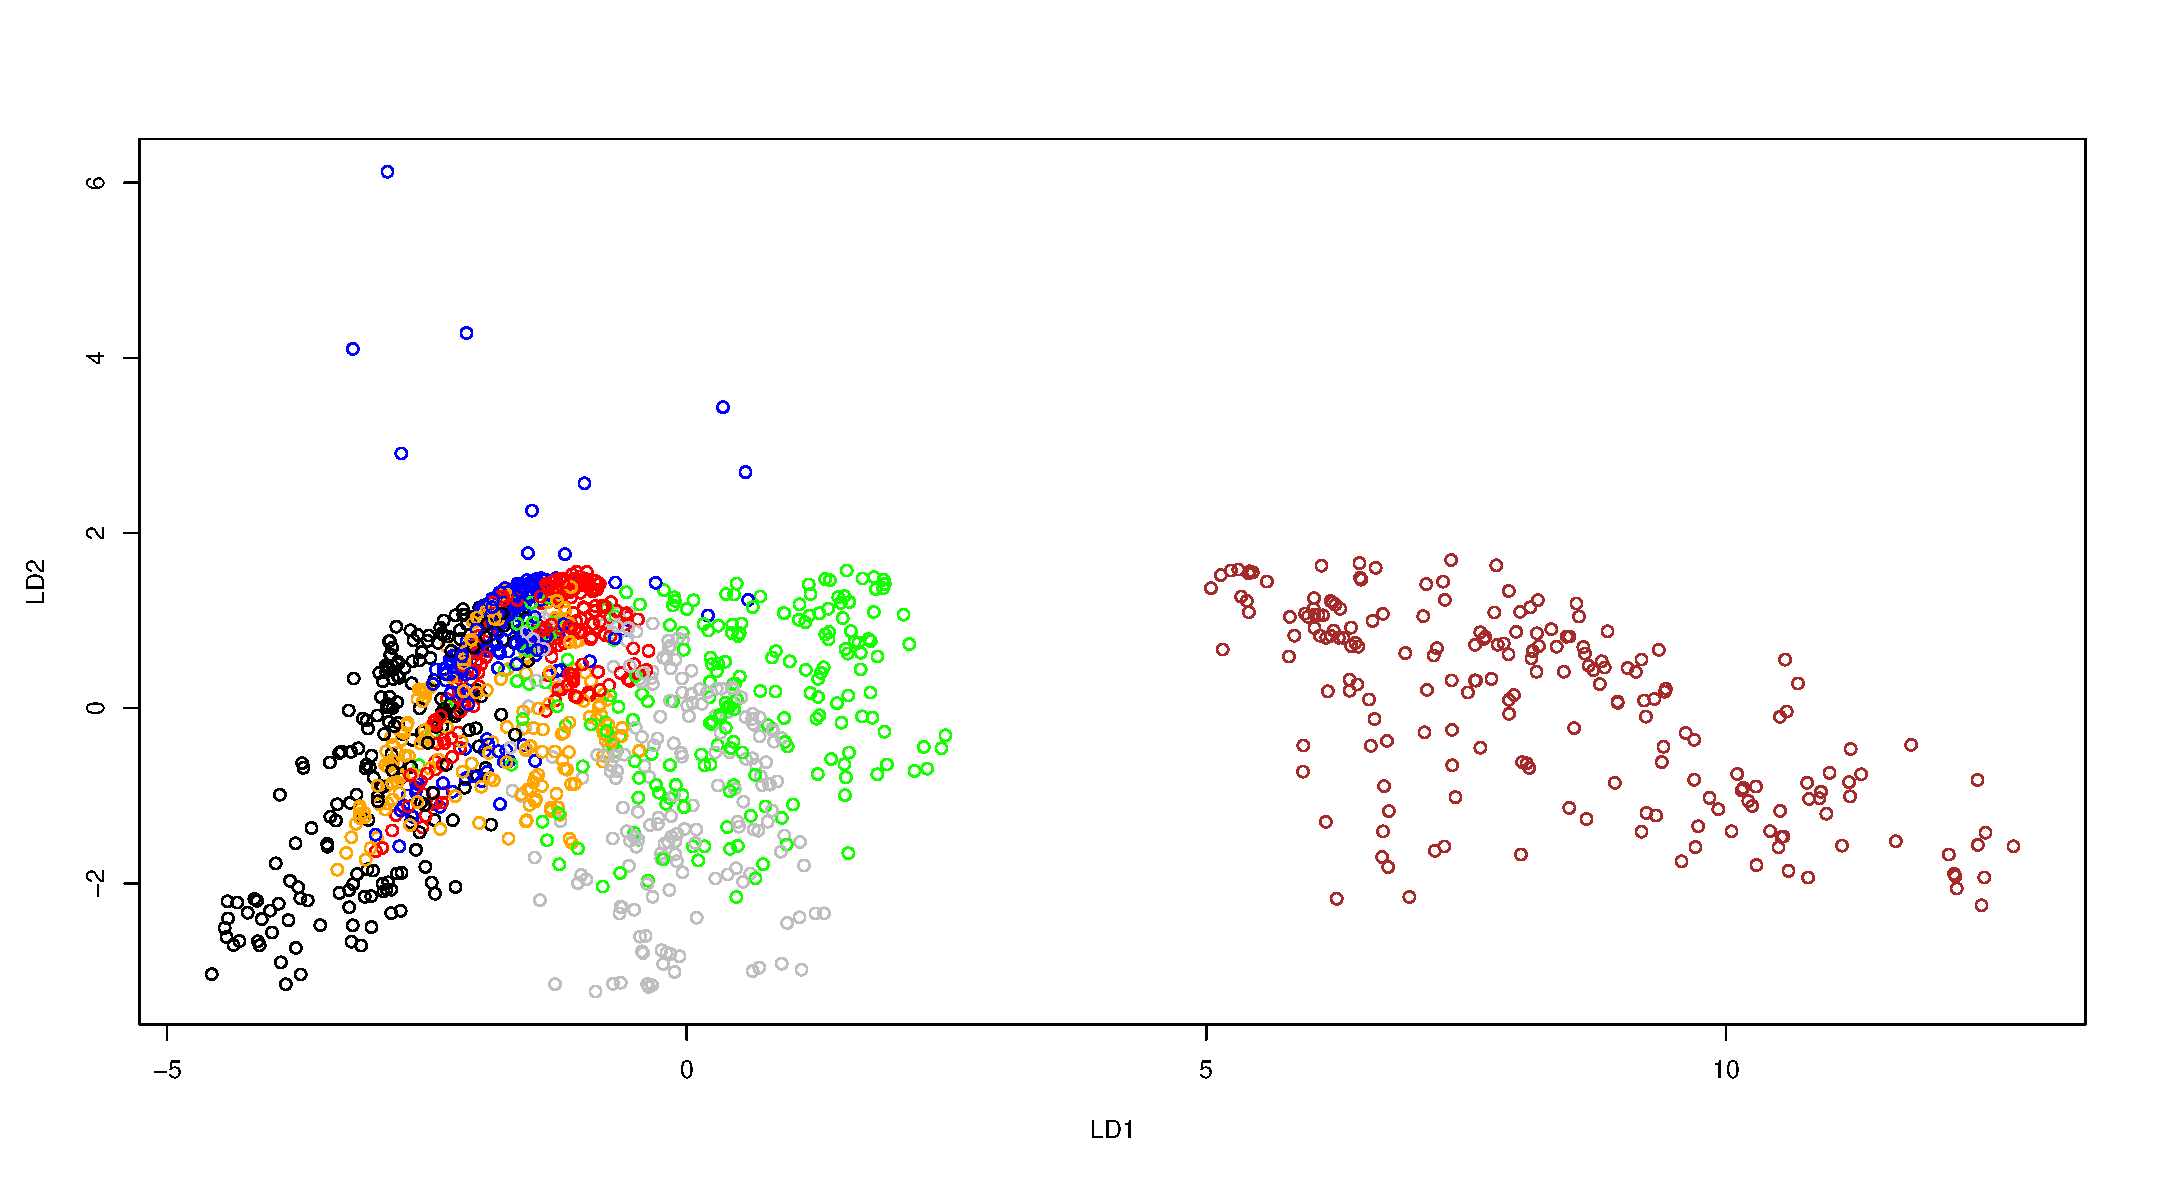
\includegraphics[width=12.1cm]{small_kpca_lda_poly_LD12.eps}
\caption{\textit{Projection of PC space onto first two LD components space (small data set). Here, the colors represent different classes: red--brickface, brown--sky, 
blue--foliage, green--cement, orange--window, grey--path, black--grass.}}
\end{figure}



\appendix

\section{Appendix: code in R}

The following is the code to generate my result: (written in R, and two libraries are used, ``kernlab'' and ``MASS'')

{\color{lightgray} \begin{verbatim}
> library(kernlab)

> polykernel <- polydot(degree=2,scale=1,offset=1)  # define polynomial kernel

> kpcaclassify(polykernel)
\end{verbatim}}

Here, ``kpcaclassify()'' is an user-defined function which is:

{\color{lightgray} \begin{verbatim}
function(mykernel) {

correction <- vector(length = 9) # define the vector which hold the result

# randomly generate training and test set 9 times, with different sizes
# and apply kernel PCA and LDA on those data set

for (i in 1:9) {
  smp_size <- floor(0.1*i*nrow(whole_data))
  set.seed(123)
  ind <- sample(seq_len(nrow(whole_data)),size=smp_size)
  trdata <- whole_data[ind,]
  tedata <- whole_data[-ind,]
  trlabel <- whole_label[ind]
  telabel <- whole_label[-ind]

  library(kernlab)
  kpc <- kpca(as.matrix(trdata),kernel=mykernel) # doing kernel PCA on training set
  eig <- eig(kpc) # find k eigenvalues who keep 90% of energy
  for (l in 1:length(eig)){
    if(sum(eig[1:l])/sum(eig) >= 0.9) {
      k <- l
      break
    }
  }
print(i)
print(k)
  k_train_data <- rotated(kpc)[,1:k] # training data projected onto kernel PCA space
  k_test_data <- predict(kpc,tedata)[,1:k] # project test set onto kernel PCA space
  
  library(MASS)
  sep <- lda(x=k_train_data,grouping=trlabel) # find the linear classifier
  pred <- predict(sep,k_test_data)$class # predict on test set by this classifier
  plot((predict(sep,k_test_data)$x)[,1:2],col = c("navy","green","blue","black","grey",
  "brown","orange","purple","yellow","red")[telabel])
  dif <- as.numeric(pred)-as.numeric(telabel)
  correction[i] <- length(which(dif==0))/length(dif) # record the accuracy
}

result <- list(correction=correction)
return(result)
}

\end{verbatim}}

For the part generating classifier, I also have my own code without using ``MASS'' library (the reason I use above code is that I can plot the data
on LDA space, so the result is visualized):

{\color{lightgray} \begin{verbatim}
vote <- matrix(0, nrow=length(telabel),ncol=7)

# use "one vs rest" strategy to build multiclass classifier (7 classes)
for (i in 1:7) {
    m1 <- colMeans(k_train_data[which(trlabel == i),])
    m2 <- colMeans(k_train_data[which(trlabel != i),])
    M <- k_train_data
# center data in class i
    M[which(trlabel == i),] <- t(t(M[which(trlabel == i),])-m1)
# center data in class M (not in i)
    M[which(trlabel != i),] <- t(t(M[which(trlabel != i),])-m2)
    Sigma <- (1/nrow(M))*(t(M) %*% M)
    Sigmainv <- solve(Sigma) # find inverse of matrix Sigma
    w <- 2*crossprod(m2-m1,Sigmainv)
    b <- crossprod(m2,Sigmainv)%*%m2-crossprod(m1,Sigmainv)%*%m1
    prediction <- k_test_data %*% t(w) - as.numeric(b)
    for (l in 1:length(telabel)) {
      if (prediction[l] > 0) vote[l,i] = vote[l,i]+prediction[l]
    }
for (i in 1:nrow(vote)) {
  pred[i] <- which.max(vote[i,])
}
\end{verbatim}}

\end{document}


